% 行列式
% 线性代数|矢量|矩阵|方阵|行列式|线性无关|置换|逆序数

% 首先介绍二阶和三阶行列式,因为最常用! 然后介绍一般行列式的计算法则及性质(必须是以后会用到的,否则不写!

行列式是线性代数中的一个重要工具,主要用于判断方阵中的所有列向量的线性无关\footnote{充分必要条件是所有行向量也线性无关}.%未完成: 证明
行列式运算的结果是一个数,若结果不为零,则线性无关,为零则线性相关. 物理中经常出现的是二阶和三阶行列式, 我们先介绍它们的性质, 然后介绍高阶的情况.

\subsection{二阶行列式的定义}
\begin{equation}\label{Deter_eq1}
\begin{vmatrix}
a_{11} & a_{12} \\
a_{21} & a_{22}
\end{vmatrix} = a_{11}a_{22} - a_{12}a_{21}
\end{equation}

\subsection{三阶行列式的定义}
\begin{equation}\label{Deter_eq2}
\begin{vmatrix}
a_{11} & a_{12} & a_{13} \\
a_{21} & a_{22} & a_{23} \\
a_{31} & a_{32} & a_{33}
\end{vmatrix}
= \leftgroup{
&a_{11}a_{22}a_{33} + a_{12}a_{23}a_{31} + a_{13}a_{21}a_{32} \\
- &a_{11}a_{23}a_{32} - a_{12}a_{21}a_{33} - a_{13}a_{22}a_{31}
}\end{equation}

我们经常把行列式中的数表叫做\textbf{矩阵}\upref{Mat}, 但本文并不涉及矩阵的性质和运算. 若将矩阵记为 $\mat A$, 则 $\mat A$ 的行列式记为 $\abs{\mat A}$.

\subsection{几何理解}
\pentry{几何矢量\upref{GVec}, 右手定则\upref{RHRul}}

\begin{figure}[ht]
\centering
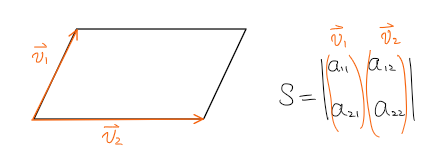
\includegraphics[width=8cm]{./figures/Deter1.png}
\caption{二阶行列式的绝对值对应平行四边形的面积} \label{Deter_fig1}
\end{figure}
如\autoref{Deter_fig1}, 二阶行列式的绝对值对应平行四边形的面积(可以认为是二维空间中的 “体积”), 若把行列式的两列看成两个几何矢量的坐标, 他们就是平行四边形的两条边. 当 $\bvec v_1$ 逆时针转动\footnote{假设转动角度小于 180°, 下同.}得到 $\bvec v_2$ 时, 行列式的值为正, 反之为负.

\begin{figure}[ht]
\centering
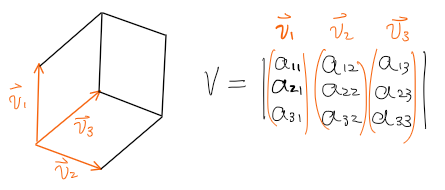
\includegraphics[width=9cm]{./figures/Deter2.png}
\caption{三阶行列式对应平行四面体的体积} \label{Deter_fig2}
\end{figure}
如\autoref{Deter_fig2}, 二阶行列式代表一个平行四面体的体积, 若把行列式的 3 列看成 3 个几何矢量的坐标, 他们就是平行四面体的 3 条边. 若 $\bvec v_1, \bvec v_2, \bvec v_3$ 的位置关系与 $x, y, z$ 轴的关系相似(符合右手定则\upref{RHRul}) 则行列式的值为正, 反之为负.

\begin{exercise}{}
请证明二阶行列式对应平行四边形的面积, 三阶行列式对应平行四面体的体积
\end{exercise}

以上两个结论也可以拓展到更高维的情况, 即 $N$ 阶行列式表示 $N$ 维空间中平行体的体积. 但由于我们还没严格定义高维空间中的体积, 先不展开.

\subsection{常见性质}
根据行列式的几何理解, 我们容易得到它的一些性质.

\begin{theorem}{ } \label{Deter_the1}
若行列式中某列全为 0, 其结果等于 0.
\end{theorem}
若平行体的某条边长等于 0, 其体积也等于 0.

\begin{theorem}{ }
若行列式中的列矢量线性相关, 其结果等于 0.
\end{theorem}
二维情况下两矢量线性相关意味着他们共线, 平行四边形面积为 0. 三维情况下线性相关意味着三个矢量共面, 平行四面体体积为 0. 高维情况也可类比.

\begin{theorem}{ }
除非行列式中某列全为 0, 或列矢量线性相关, 行列式的值不为 0.
\end{theorem}

\begin{theorem}{ }
矩阵的任意一列乘以常数,行列式的值也要乘以该常数.
\end{theorem}
按照几何理解, 将平行体任意一条边长乘以一个常数, 它的体积也需要乘以该常数. 至于定理中的正负号, 可以由各阶行列式的定义证明(留做练习).

\begin{theorem}{ }
把矩阵的第 $i$ 列叠加上 “第 $j$ 列乘任意常数”,行列式的值不变.
\end{theorem}
以平行四边形为例, 由于其体积是底乘以高, 令 $\bvec v_1$ 为底, $\bvec v_2$ 在垂直于 $\bvec v_1$ 方向的投影为高, 则将 $\bvec v_2$ 变为 $\bvec v_2 + \lambda \bvec v_1$ ($\lambda$ 为常数)后高不变, 所以面积不变. 三维情况和高维情况同理.

\begin{theorem}{ }
将行列式的两列交换, 结果取相反数.
\end{theorem}
对二阶和三阶行列式, 无论从代数还是几何上都容易得到这个结论. 对于任意阶的情况, 该操作会给每一项增加一个逆序数(见下文), 导致结果取相反数.

\begin{theorem}{ }
矩阵\textbf{转置}(将所有 $a_{i,j}$ 与 $a_{j,i}$ 交换\upref{Mat})后行其列式的值不变.
\end{theorem}
这个定理没有显然的几何理解, 可以直接用代数定义证明(\autoref{Deter_eq1} 和\autoref{Deter_eq2}, 以及下文的\autoref{Deter_eq4}). 根据这个定理, 以上凡是涉及到 “行” 的定理和说明, 都可以替换为 “列”, 请读者自行回顾一次.

\subsection{高阶行列式的定义}

$N$ 阶行列式($N$ 为正整数\footnote{一阶行列式定义为 $\abs{a_{11}}=a_{11}$, 虽然几乎从不被使用})共有 $N!$ 项,每一项都是 $N$ 个矩阵元的乘积\footnote{高阶行列式的计算较为复杂, 可通过数学软件计算, 详见 Matlab,Mathematica 和 Wolfram Alpha 的计算方法.%未完成: 链接
}. 每一项中的 $N$ 个矩阵元的行数和列数各不相同, 我们既可以在每一项中按照行标来排序,也可以按照列标,我们选用前者. 排序后,行列式展开后的任意一项可记为(先不考虑前面的 $\pm$ 号)
\begin{equation}\label{Deter_eq3}
\prod_{i=1}^N a_{i,P_n(i)} = 
a_{1,P_n(1)} \vdot a_{2,P_n(2)} \dots
\end{equation}
其中列标 ${P_n}(i)$ 是数列 $1,2 \dots N$ \textbf{置换}(用某种顺序排列)后的第 $i$ 个数,显然该数列共有 $N!$ 种不同的排列,这里用 $n$ 表示第 $n$ 种排列,也表示行列式展开的第 $n$ 项.

现在来考虑\autoref{Deter_eq3} 前面的 $\pm$ 号.这由 $P_n$ 的\textbf{逆序数} 决定, 逆序数的定义为
\begin{equation}
\sum_{i=2}^N \text{满足}\, P_n(i) < P_n(j) \,\, (j<i) \,\text{的个数} 
\end{equation}
若逆序数为偶数,则前面加正号, 奇数则加负号. 若根据 $P_n$ 对应的符号定义数列 $S_n$ (取值 $1$ 或 $-1$),则 $N$ 阶行列式的公式为
\begin{equation}\label{Deter_eq4}
\begin{vmatrix}
a_{11} & \cdots & a_{1n} \\
\vdots & \ddots & \vdots \\
a_{n1} & \cdots & a_{nn}
\end{vmatrix}
= \sum_{n=1}^{N!} S_n \prod_{i=1}^N a_{i,P_n(i)}
\end{equation}


